\documentclass{standalone}
\usepackage{graphicx}	
\usepackage{amssymb, amsmath}
\usepackage{color}

\usepackage{tikz}
\usetikzlibrary{intersections, backgrounds, math}
\usepackage{pgfmath}

\definecolor{light}{RGB}{220, 188, 188}
\definecolor{mid}{RGB}{185, 124, 124}
\definecolor{dark}{RGB}{143, 39, 39}
\definecolor{highlight}{RGB}{180, 31, 180}
\definecolor{light_teal}{RGB}{107, 142, 142}
\definecolor{mid_teal}{RGB}{72, 117, 117}
\definecolor{dark_teal}{RGB}{29, 79, 79}
\definecolor{gray10}{gray}{0.1}
\definecolor{gray20}{gray}{0.2}
\definecolor{gray30}{gray}{0.3}
\definecolor{gray40}{gray}{0.4}
\definecolor{gray60}{gray}{0.6}
\definecolor{gray70}{gray}{0.7}
\definecolor{gray80}{gray}{0.8}
\definecolor{gray90}{gray}{0.9}
\definecolor{gray95}{gray}{0.95}

\begin{document}

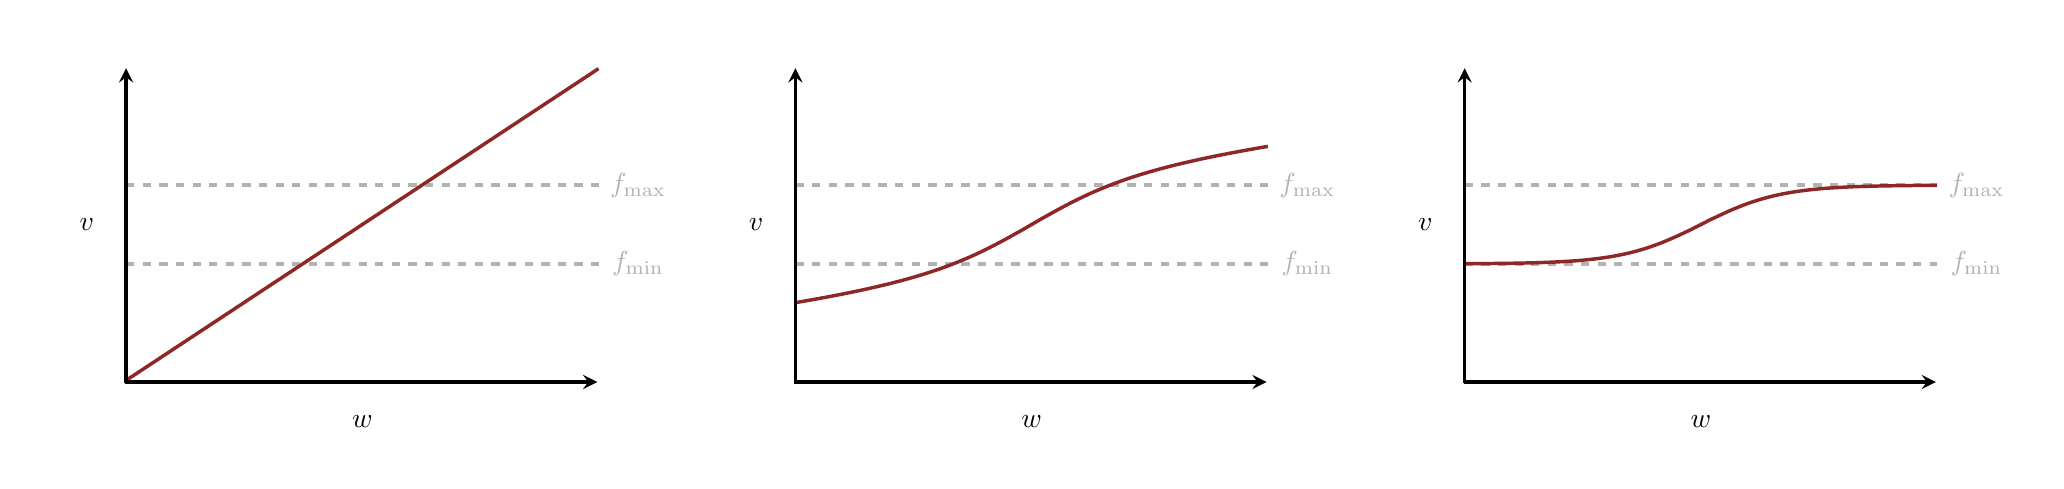
\begin{tikzpicture}[scale=1.0]

  \pgfmathsetmacro{\ys}{0.66};
  
  \pgfmathsetmacro{\lambdamix}{0.0};
  \begin{scope}[shift={(0, 0)}]
    \fill[white] (-4.25, -3) rectangle (4.25, 2.5);
        
    \draw[gray70, dashed, line width=1.5] (-3, 0.5) -- (3, 0.5);
    \node[gray70] at (3.5, 0.5) { $f_{\max}$ };
    
    \draw[gray70, dashed, line width=1.5] (-3, -0.5) -- (3, -0.5);
    \node[gray70] at (3.5, -0.5) { $f_{\min}$ };
    
    \draw[domain={0.01:6}, smooth, samples=50, line width=1.25, variable=\x, color=dark] 
      plot ({\x / 2},{0.5 * exp((1 - \lambdamix) * ln(\ys * \x) + \lambdamix * ln(2.0 / (1 + exp(-\x)) - 1))});

    \draw[domain={-0.01:0.01}, smooth, samples=5, line width=1.25, variable=\x, color=dark] 
      plot ({\x},{\ys * \x});

    \draw[domain={-6:-0.01}, smooth, samples=50, line width=1.25, variable=\x, color=dark] 
      plot ({\x / 2},{-0.5 * exp((1 - \lambdamix) * ln(-\ys * \x) + \lambdamix * ln(2.0 / (1 + exp(\x)) - 1))});


    \draw [->, >=stealth, line width=1.25] (-3.00, -2.015) -- +(0, 4);
    \draw [->, >=stealth, line width=1.25] (-3.015, -2.00) -- +(6, 0);
    
    \node at (-3.5, 0) { $v$ };
    \node at (0, -2.5) { $w$ };
  \end{scope}

  \pgfmathsetmacro{\lambdamix}{0.5};
  \begin{scope}[shift={(8.5, 0)}]
    \fill[white] (-4.25, -3) rectangle (4.25, 2.5);
        
    \draw[gray70, dashed, line width=1.5] (-3, 0.5) -- (3, 0.5);
    \node[gray70] at (3.5, 0.5) { $f_{\max}$ };
    
    \draw[gray70, dashed, line width=1.5] (-3, -0.5) -- (3, -0.5);
    \node[gray70] at (3.5, -0.5) { $f_{\min}$ };
    
    \draw[domain={0.01:6}, smooth, samples=50, line width=1.25, variable=\x, color=dark] 
      plot ({\x / 2},{0.5 * exp((1 - \lambdamix) * ln(\ys * \x) + \lambdamix * ln(2.0 / (1 + exp(-\x)) - 1))});

    \draw[domain={-0.01:0.01}, smooth, samples=5, line width=1.25, variable=\x, color=dark] 
      plot ({\x},{\ys * \x});

    \draw[domain={-6:-0.01}, smooth, samples=50, line width=1.25, variable=\x, color=dark] 
      plot ({\x / 2},{-0.5 * exp((1 - \lambdamix) * ln(-\ys * \x) + \lambdamix * ln(2.0 / (1 + exp(\x)) - 1))});


    \draw [->, >=stealth, line width=1.25] (-3.00, -2.015) -- +(0, 4);
    \draw [->, >=stealth, line width=1.25] (-3.015, -2.00) -- +(6, 0);
    
    \node at (-3.5, 0) { $v$ };
    \node at (0, -2.5) { $w$ };
  \end{scope}
  
  \pgfmathsetmacro{\lambdamix}{1.0};
  \begin{scope}[shift={(17, 0)}]
    \fill[white] (-4.25, -3) rectangle (4.25, 2.5);
        
    \draw[gray70, dashed, line width=1.5] (-3, 0.5) -- (3, 0.5);
    \node[gray70] at (3.5, 0.5) { $f_{\max}$ };
    
    \draw[gray70, dashed, line width=1.5] (-3, -0.5) -- (3, -0.5);
    \node[gray70] at (3.5, -0.5) { $f_{\min}$ };
    
    \draw[domain={0.01:6}, smooth, samples=50, line width=1.25, variable=\x, color=dark] 
      plot ({\x / 2},{0.5 * exp((1 - \lambdamix) * ln(\ys * \x) + \lambdamix * ln(2.0 / (1 + exp(-\x)) - 1))});

    \draw[domain={-0.01:0.01}, smooth, samples=5, line width=1.25, variable=\x, color=dark] 
      plot ({\x},{\ys * \x});

    \draw[domain={-6:-0.01}, smooth, samples=50, line width=1.25, variable=\x, color=dark] 
      plot ({\x / 2},{-0.5 * exp((1 - \lambdamix) * ln(-\ys * \x) + \lambdamix * ln(2.0 / (1 + exp(\x)) - 1))});


    \draw [->, >=stealth, line width=1.25] (-3.00, -2.015) -- +(0, 4);
    \draw [->, >=stealth, line width=1.25] (-3.015, -2.00) -- +(6, 0);
    
    \node at (-3.5, 0) { $v$ };
    \node at (0, -2.5) { $w$ };
  \end{scope}
    
\end{tikzpicture}

\end{document}  